\documentclass[tikz,border=5pt]{standalone}
\usepackage{amsmath}
\usetikzlibrary{arrows.meta,positioning,fit,calc}

\begin{document}
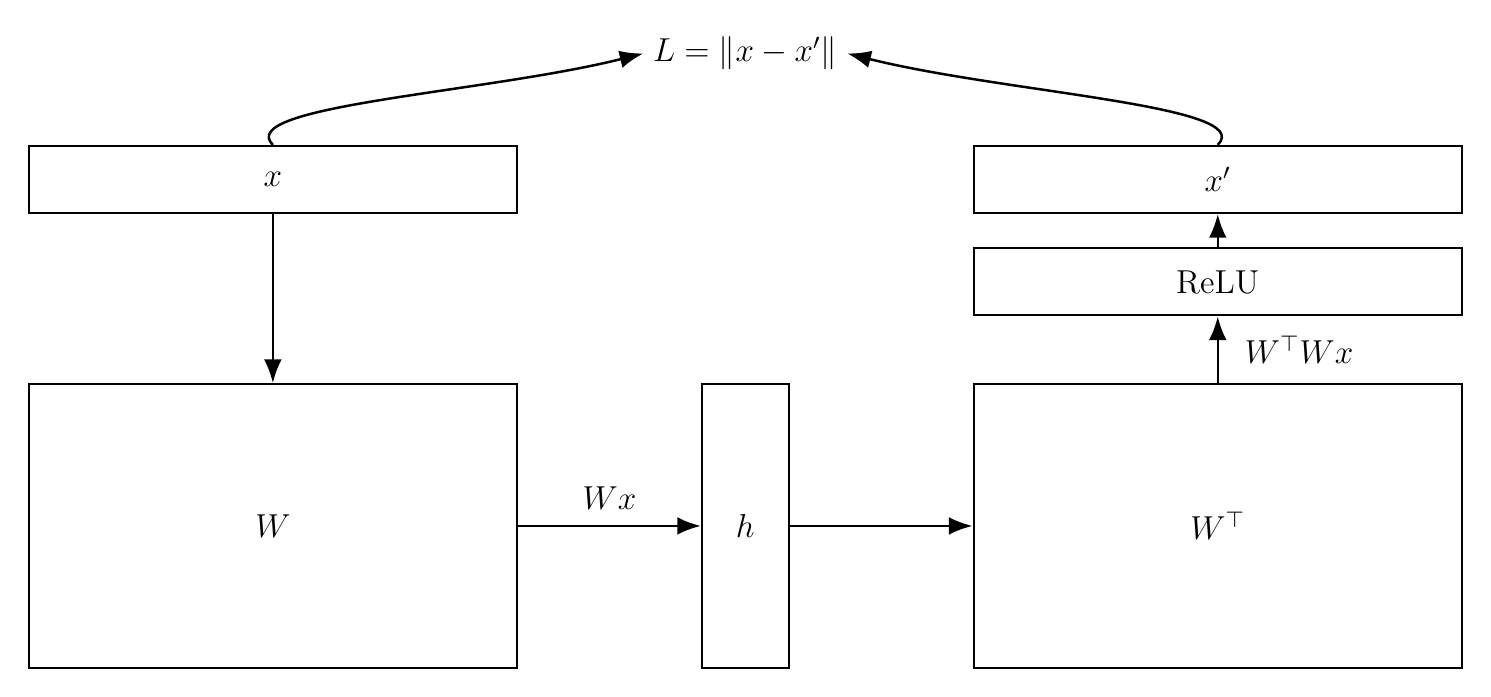
\begin{tikzpicture}[font=\large]
  %----- styles
  \tikzset{
    box/.style  ={draw,thick,minimum width=6.2cm,minimum height=3.6cm,align=center},
    slim/.style ={draw,thick,minimum width=1.1cm,minimum height=3.6cm,align=center},
    var/.style  ={draw,thick,minimum width=6.2cm,minimum height=0.85cm}, % rectangular, same width as W
    slab/.style ={draw,thick,minimum width=6.2cm,minimum height=0.85cm}, % same width as W
    arrow/.style={-{Latex[length=3mm]},line width=0.9pt}
  }

  %----- nodes
  % left side
  \node[var] (x)  at (-6, 3.8) {$x$};         
  \node[box] (W)  at (-6,-0.6) {$W$};
  % middle latent
  \node[slim] (h) at ( 0,-0.6) {$h$};
  % right side
  \node[box] (Wt)   at ( 6,-0.6) {$W^{\top}$};
  \node[slab] (relu)at ( 6, 2.5) {ReLU};
  \node[var] (xp)   at ( 6, 3.8) {$x'$};

  %----- connections
  \draw[arrow] (x.south) -- (W.north);
  \draw[arrow] (W.east) -- node[above=2pt] {$Wx$} (h.west);
  \draw[arrow] (h.east) -- (Wt.west);

  % Arrow W^T -> ReLU, with label
  \draw[arrow] (Wt.north) -- (relu.south) node[midway,right=6pt] {$W^{\top} W x$};

  \draw[arrow] (relu.north) -- (xp.south);

  %----- top loss label and concave-downward arrows
  \node (loss) at (0,5.4) {$L=\lVert x - x' \rVert$};
  \draw[arrow] (x.north) .. controls +(-0.5,0.5) and +(-2,-0.5) .. (loss.west);
  \draw[arrow] (xp.north) .. controls +(0.5,0.5) and +(2,-0.5) .. (loss.east);
\end{tikzpicture}
\end{document}
